\documentclass[a4paper]{article}
\usepackage[margin=10mm]{geometry}
\usepackage {array, tikz, amssymb}
\centering

\tikzset{
  pics/mynode/.style args={#1,#2,#3}{
     code={
     \draw (-1,0) arc (180:360:1);
     \draw (1,0) arc (0:180:1 and 2);
     \draw [rounded corners=2 ] (0,2) -- (0.5,2.5) -- (-0.5,2.5) -- cycle;
     % How do I scale bag to 30%?
     \node[#3] (#1) at (1,1) {#2};
     }
  }
}


\begin{document}
\begin{center}
\begin{tabular}{ m{8cm}  m{0.5cm}  m{8cm} }

3) & & 4) \\

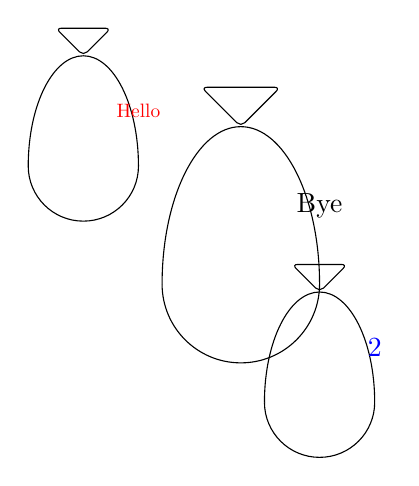
\begin{tikzpicture}
      \draw (3,0) pic[scale=0.7]{mynode={1,2,blue}};
      \draw (0,3) pic[scale=0.7, transform shape]{mynode={B, Hello, red}};
      \draw (2,1.5) pic{mynode={C, Bye,}};
      %\draw[thick, blue] (A)--(B)--(C)--(A);
  \end{tikzpicture} & & \\

\end{tabular}
\end{center}
\end{document}